\documentclass[12pt,a4paper,oneside]{article}
\usepackage{titlepic}
\usepackage[utf8]{inputenc}
\usepackage{graphicx}
\usepackage[left=1.1in,right=1.1in, top=1in, bottom= 1in]{geometry}
\usepackage{amsfonts}
\usepackage{amssymb}
\usepackage{amsmath}
\usepackage{fancyhdr}
\usepackage{hyperref}
\usepackage{etoolbox}
\usepackage[nottoc]{tocbibind}
\usepackage{appendix}
\usepackage{multicol}
\usepackage{leftidx}
\graphicspath{{figures/}}
\usepackage{ragged2e}
\usepackage{mathtools}
\usepackage{units}
\usepackage{float}
\usepackage{subcaption}
\usepackage{commath}
\usepackage{comment}

\usepackage{amsthm}
 
\theoremstyle{definition}
\newtheorem{definition}{Definition}[section]

\newtheorem{theorem}{Theorem}

\usepackage[none]{hyphenat} % Avoids to go out of margin

\usepackage{subfiles}

\usepackage{minted}
\usemintedstyle{xcode}
\setminted{breaklines,fontsize=\footnotesize,frame=single}

\newcounter{freqcounter}
\newcommand{\req}[1]{%
	\textbf{FR\ref*{#1}}\refstepcounter{freqcounter}\label{#1}%
}
\newcommand{\reqref}[1]{%
	\hyperref[#1]{[FR\ref*{#1}]}%
}

\newcounter{nfreqcounter}
\newcommand{\nreq}[1]{%
	\textbf{NFR\ref*{#1}}\refstepcounter{nfreqcounter}\label{#1}%
}
\newcommand{\nreqref}[1]{%
	\hyperref[#1]{NFR\ref*{#1}}%
}

\newcommand{\ReqItemStyle}[1]{\textbf{#1}}
\newcommand{\ReqItem}[2]{\item[\req{#1}] \ReqItemStyle{#2}}
\newcommand{\NReqItem}[2]{\item[\nreq{#1}] \ReqItemStyle{#2}}

% --------------------------------------------- %

\title{Derp}	                                    % Title
\author{Author Name}				                % Authors separated by \\
\date{\today}									    % Date

% Font size of figure smaller than normal size:
\usepackage{caption}
\captionsetup[figure]{font=small}
%\captionsetup[table]{font=small}

%\usepackage{setspace} % double spacing
\linespread{1.2}

\makeatletter
\let\thetitle\@title
\let\theauthor\@author
\let\thedate\@date
\makeatother

\begin{document}

\begin{titlepage}
	\centering
	\vspace*{0.5 cm}
	\includegraphics[scale = 0.75]{figures/SapienzaLogo.pdf}\\[1.0 cm]	% University Logo

	{ \fontsize{20.74pt}{18.5pt}\selectfont\bfseries \thetitle \par } % Title

	\vspace*{0.25cm}
	\textsc{\Large Blockchain and Distributed Ledger Technologies 2022}\\[0.5 cm] % Course Name

	\vspace*{2.6cm}
	\hspace{3em}
	\begin{minipage}{0.3\textwidth} % 0.4
		\begin{flushleft} \large
			\textbf{Andrea Reale}\\
			2003188\\
		\end{flushleft}
	\end{minipage}~
	\hspace{3em}
	\begin{minipage}{0.3\textwidth} %0.4
		\begin{flushright} \large
			\begin{minipage}{1\textwidth}
				\begin{flushleft} \large
					\textbf{Matteo Gioia} \\
					1995989
				\end{flushleft}
			\end{minipage}
		\end{flushright}
	\end{minipage}\\[3.85 cm]

	\vspace{8cm}
	\rule{\linewidth}{0.2 mm} \\[0.3 cm]
	Academic Year 2022/2023
\end{titlepage}

\newpage
\tableofcontents
\newpage


%glossary in latex
%context: a context in phoenix is a module that is used to group related functionality.


\section{Introduction}

The rise of e-commerces revolutionized the way we buy and sell products. Before the creation of such platforms, there was no way to verify the quality of a product, as gathering feedback from previous customers was pretty much impossible.
This issue became one of the main selling points of e-commerces, as they provided a way for users to share their experience with a product and for others to make an informed decision before buying it.
However, the lack of a centralized authority to verify the authenticity of the reviews has led to the proliferation of fake reviews. For example, it is not uncommon for vendors to ask to leave fake reviews in exchange for money or a free product, or for users to leave negative feedbacks in order to boycott a specific vendor. On top of that, there is no way to verify whether the content of the review is what the original poster had actually written. \\
The goal of D.E.R.P. is to address all of these challenges while building a platform that incentivizes its customers to leave honest reviews and interact with the website.

\paragraph{Responsibilities} The development of the app (backend, frontend, smart contract) was carried on by all team members equally. However, there are a few key elements which were personally ideated/curated by a specific team member, as listed below:
\begin{itemize}
	\item Andrea Reale: oracle to check whether user has bought news product, docker setup
	\item Matteo Gioia: documentation stub, slides
\end{itemize}

\paragraph{Outline of the report TO CORRECT} This report is organized as follows:
\begin{itemize}
	\item The first section provides a brief overview of the background of the project, including a brief introduction to the blockchain technology and the e-commerce domain.
	\item The second section describes the context of the DApp, including the main problems that we are trying to solve and the rationale behind the use of a blockchain.
	\item The third section describes the architecture of the DApp, including the functional requirements, the use-case diagrams, the sequence diagrams, the backend, the frontend and the smart contract.
	\item The fourth section describes the implementation details of the DApp, including visual examples.
	\item The fifth section describes the known issues of the DApp.
	\item The last section provides a conclusion of the project.
\end{itemize}

\section{Background}
% Blockchain: history, rationale, concepts...

The idea of blockchain was first suggested in 1991 by Stuart Haber and W. Scott Stornetta, who described a system that would allow users to timestamp a document and store it in a distributed way [MT] Modern blockchains have gone a long way from this initial concept, and they are now used in a wide range of applications, from cryptocurrencies to supply chain management. A blockchain is in fact a \textbf{protocol} by definition and this means that there is no standard implementation but rather a multitude of them.
During the recent years, the Bitcoin and Ethereum ones rose in popularity among the general public and are now widely adopted and used. As such, they can be used to present the main concepts of a blockchain and how they are implemented in practice. \\

\paragraph{Blockchain} A blockhain, as the name suggests, is a collection of \textbf{blocks} that are \textbf{linked together in a chain}. This link is achieved, for instance, by including the \textbf{hash} of the previous block inside the next one. The inside of each block contains \textbf{transactions} between \textbf{addresses} on the chain plus some extra information, such as the \textbf{timestamp} of the block. A blockchain is generally \textbf{immutable} and can be of four different types, as shown in the following diagram: 
\begin{figure}
  \centering
  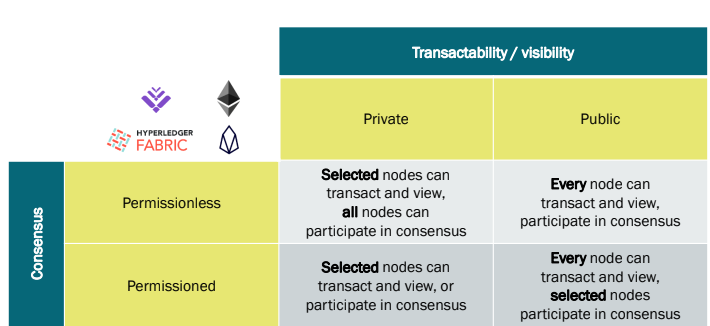
\includegraphics[width=0.8\textwidth]{figures/bt_types.png}
  \caption{Types of blockchains - from lecture slides by Prof. Di Ciccio}
  \label{fig:blockchain_types}
\end{figure}
Most blockchains are public and permissionless, and as such all the nodes have the ability to see the full history of the transactions.


\paragraph{Nodes} Nodes are a building block of every decentralized protocol. Depending on the nature of the blockchain, we can identify two nomenclatures for them:
\begin{itemize}
  \item PoW: \textbf{miners} - each node has the goal to compute the PoW for the next block and add it to the chain;
  \item PoS: \textbf{validators} - each node has the goal to validate the next block and add it to the chain.
\end{itemize}
Nodes can also cover other roles, for example veryfing the headers for the next blocks, thus speeding up the network, or only run ... \\

\paragraph{Proofs} In order for a block to be added to a blockchain, its \textbf{proposer} has to have some kind of \textbf{proof} for the inclusion. This proof can either be \textbf{expensive to compute}, like in the \textbf{Proof of Work} mechanism of Bitcoin, or \textbf{require the user to put something at stake}, as in the \textbf{Proof of Stake} of Ethereum. The trend this days is going towards the utilisation of \textbf{PoS} blockchains, as they tend to be less expensive and more scalable. It must be noted that there are other mechanism for proving the \textbf{validity} of a block, like \textbf{Proof of Time, Proof of Randomness} and so on. \\

\paragraph{pseudonimity} Contrary to popular belief, most blockchains don't grant full anonimity. In fact, it is more common for users to be \textbf{pseudonimous}. The only information that is shared is their \textbf{public key} so their identity is not known, but the transactions that they perform are. This key feature allows for \textbf{anonymity} and \textbf{transparency} at the same time. Note that some blockchains - like Monero's - do actually grant anonimity. In the case of Bitcoin, instead, a user that inadvertedly leaks their public key would de-anonimize themselves.\\

\paragraph{Smart contracts and Gas} Some blockchain implementations, like Ethereum, offer a \textbf{Turing complete language} which can be used to \textbf{write pieces of code that run on the blockchain itself}. These pieces of code are called \textbf{smart contracts} and they can be used to implement a wide range of applications, as they also posses \textbf{their own storage}. Their key characteristic is that they are \textbf{immutable}: once created, there is no way to change them. On top of that, after calling a function there is no guarantee that the code is eventually reaching a halt! For this reason, there exist control mechanisms such as \textbf{gas}. Gas is exchanged for \textbf{Weis} at a price decided by the user when making  transactions and will be used to fuel the code execution, eventually leading to a stop when it finishes. In order to keep the price of gas stable and the Ethereum network functioning, additional measures, such as part of the gas being burnt in every transaction, are put in place. \\

\paragraph{NFTs} Smart contracts allow for the creation of tokens, i.e. internal assets which can be bought, sold and exchanged between users. These tokens can be:
\begin{itemize}
  \item \textbf{fungible}: they are all the same and can be exchanged at a 1:1 ratio;
  \item \textbf{non-fungible}: they are different and can't be exchanged at a 1:1 ratio;
  \item \textbf{semi-fungible}: they could be fungible until redeemed or expired.
\end{itemize}
During the last years, NFTs became particularly popular, as they can be used to represent digital assets such as artworks, music, videos and so on. The most famous example is probably the \textbf{CryptoPunks} collection, which is a set of 10,000 unique images.\\


\subsection{E-commerce}
% Application domain

\section{Context of the D-App}
% Aim of the DApp
The goal of D.E.R.P. is to solve the problem of fake reviews on e-commerce platforms. The main idea is to use a blockchain to store the reviews and verify their authenticity. Other features will include the possibility to interact with the reviews and customize the user profile. A full list of the features is available in the requirements section. \\
The main problems that we tackle are:
\begin{itemize}
	\item Authenticity: the hash of the review should be stored on-chain, so that it's authenticity can be verified.
	\item Boycotting: users shouldn't be able to boycott a product by leaving fake reviews.
	\item Over the counter scams: vendors shouldn't be able to bribe users to leave fake reviews.
	\item Self promoting: vendors shouldn't be able to buy/generate reviews through fake accounts.
\end{itemize}

We also want to provide a place for users to customize their profile, such as a personal page. This will increase the engagement of the users and will incentivize them to keep interacting with the platform. \\
Ideally, this platform should solve entirely the problem of fake reviews, however we are aware that this is not possible unless other requirements are met. For an extensive list of know issues, please refer to the appropriate section.

\begin{figure}[H]
	\centering
	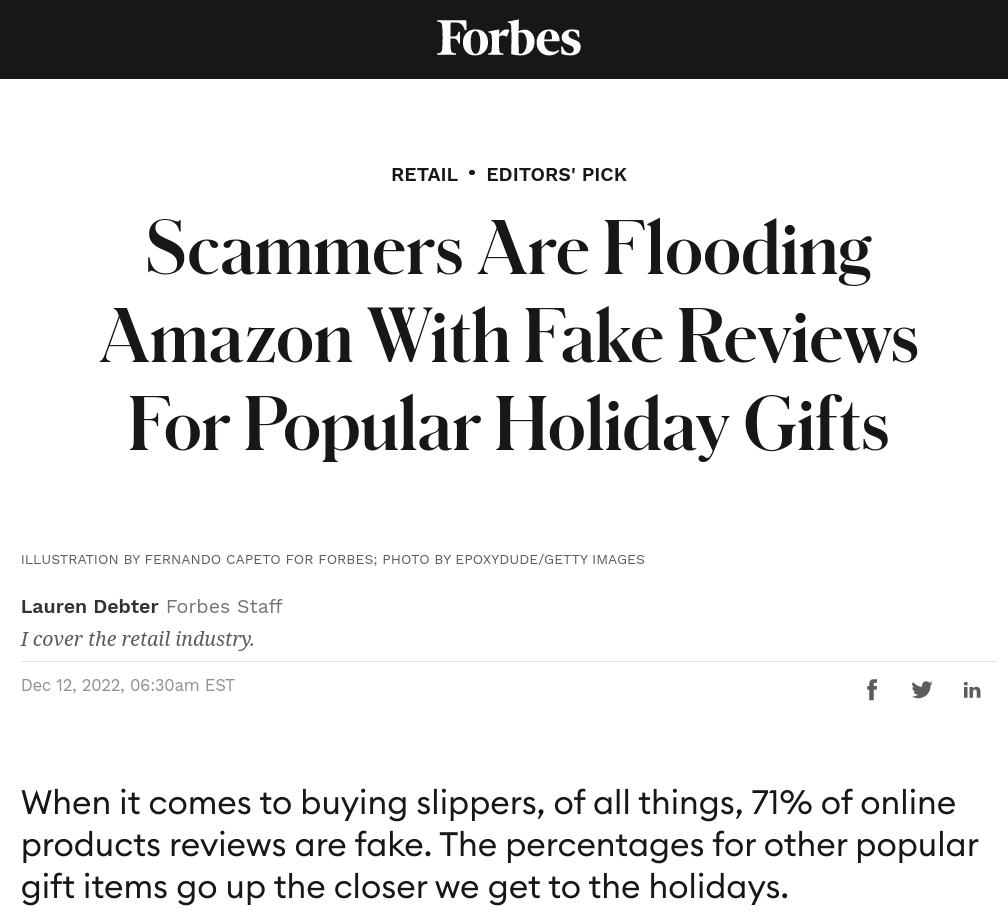
\includegraphics[width=.49\linewidth]{figures/forbes-amazon.png}
	\caption{Fake reviews are a serious problem for consumers and e-commerce sites. (Photo courtesy of Forbes.)}
\end{figure}

\subsection{Why using a blockchain?}
We make use of the Ethereum network, which is a public permissionless blockchain. This decision was made because we don't trust neither the user, which makes reviews, nor the seller of a product: one or both of them may be trying to publish a fake review and we want to prevent that.

Another reason for building a dApp was the fact that we want to be independent from a trusted third party to host the reviews: it's not possible to know whether the reviews are being manipulated in some way, for example by hiding the bad ones, which defeats the purpose of such a platform. Since a blockchain by definition is immutable it's not possible to manipulate what gets published, even more so in a public permissionless one like Ethereum: each node knows the state of the chain after each transaction, including the reviews that are stored and their authors.

\begin{figure}[H]
	\centering
	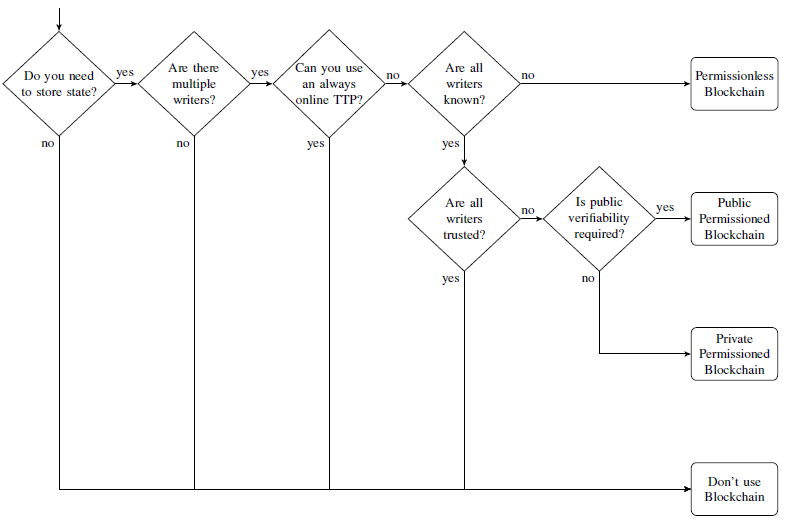
\includegraphics[width=0.75\linewidth]{figures/should-use-blockhain.png}
\end{figure}

% https://nymag.com/intelligencer/2022/07/amazon-fake-reviews-can-they-be-stopped.html
% https://www.forbes.com/sites/laurendebter/2022/12/12/scammers-are-flooding-amazon-with-fake-reviews-for-popular-holiday-gifts/
%
% An e-store, in fact, could intentionally hide/modify reviews!
% A public permissionless blockchain is a good fit for these requirements.

\subsection{Functional and Non-Functional Requirements}

In this section we define a list of functional and non-functional requirements for D.E.R.P.

\begin{itemize}
	\ReqItem{req:profile}{A user should be able to make a profile on the website.}

	In order to save their email, profile items and such, the user should register to the website.

	\ReqItem{req:claim-rt}{A user should be able to claim review tokens for a product that they have bought previously.}

	After buying a product from an external store, the user should be able to claim the right amount of review tokens for that product.

	\ReqItem{req:make-review}{A user should be able to make a review for a product that they have bought previously.}

	After buying a product from an external store, the user should see that product as available for reviewing and be able to review it.

	\ReqItem{req:interact}{A user should be able to interact with other users' reviews.}

	For example by seeing other reviews and upvoting them if they have enough review tokens.

	\ReqItem{req:browse-products}{A user should be able to browse products on the website.}

	The website should have a section that lists products that the contract knows about.

	\ReqItem{req:buy-items}{A user should be able to buy profile items with profile tokens.}

	\ReqItem{req:use-items}{A user should be able to apply profile items to customize their profile.}

	It requires the backend to store which customizations are applied for which user (see \reqref{req:profile}).

	\ReqItem{req:earn-pt}{A user should be able to earn profile tokens.}

	Needed by \reqref{req:buy-items} and \reqref{req:use-items}.

	\NReqItem{nreq:low-cost}{The operations made by the user should be cheap.}

	To incentivize the users to interact with the platform, we want their experience to be as frictionless as possible. This includes paying the lowest possible amounts of gwei in order to perform the various operations (\reqref{req:claim-rt}, \reqref{req:make-review}, \reqref{req:interact}).
	This implies that the platform operators should absorb some of the costs for interacting with the smart contract and reduce as much as possible the gas cost of the contract.

	\NReqItem{nreq:security}{Prevent review fraud as much as possible.}

	The reviews should be as truthful as possible: the cost of making a fake review should discourage malicious users.
	This means providing review authenticity, prevent self promoting and defend against boycotting.
	It should be noted that preventing over the counter scams is impossible without using any shop that implements protocols similar to the ones used in this project.
\end{itemize}

\subsection{Tech stack}

The technology stack used in the project is the following:
\begin{itemize}
	\item \textbf{Backend}: Phoenix (Elixir framework), PostgreSQL (Database)
	\item \textbf{Frontend}: Phoenix, Javascript, Bootstrap 5, Web3.js (interaction with smart contract), Alpine.js (dynamic frontend)
	\item \textbf{Smart contract}: Solidity, Truffle Suite, IPFS
	\item \textbf{Tooling}: Docker, Git
	\item \textbf{Fake shop}: Deno
\end{itemize}

The backend is written in Elixir and the CRUD were autogenerated with the help of the Phoenix framework. The frontend is also written in Phoenix and Javascript, and the interactions with the smart contract are handled with Web3.js. The smart contract is written in Solidity and it is deployed on a local node of the Ethereum blockchain, simulated with Truffle.

To make the oracle code work, we expect external shops to implement a simple HTTP API for checking if an user bought a product. We simulate this in what we call the ``fake shop'' which has store identifier ``0''.

For what regards the tooling, we created 4 containers: one for the shop server, one for truffle, one for IPFS and one for PostgreSQL. Github was used for managing the code and the project.
For an extensive list of the libraries used in the project and for a quick startup guide, please refer to the github repository that can be found at this link \url{among.us}.

\newpage
\section{Architecture}

This section is dedicated to discussing the architectural details of the DApp. In particular, we will discuss the use-case diagrams, the sequence diagrams, the backend, the frontend and the smart contract.

\subsection{Use-case diagrams}

% \begin{figure}[h]
%     \includegraphics[width=0.75\linewidth]{assets/Use Case Diagram.svg}
% \end{figure}

In this section we show the main use case diagram of our app. Since the interactions are relatively simple, we managed to fit everything in a single diagram. In fact, we only have 3 actors: the users (reviewers), the smart contract and the token themselves.

\begin{figure}[ht]
	\centering
	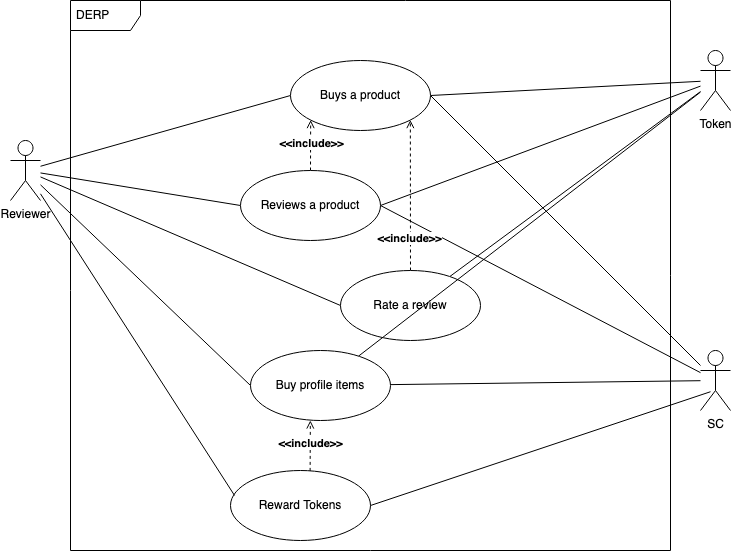
\includegraphics[scale=0.5]{figures/uc_drawio.png}
	\caption{Use case diagram}
	\label{fig:use_case}
\end{figure}


\subsection{Component Diagram}

The development of the project involved many technologies, that are shown in the following diagram.
It's important to note that for local development we used Podman (Docker) containers for the database, fake shop, truffle and IPFS. This allowed us to work easily with them in a controller environment, without having to care about possible inconsistencies in the development machines.

\begin{figure}[H]
	\centering
	\includegraphics[width=\linewidth]{figures/component}
	\caption{A basic component diagram of the various pieces of software involved in the project.}
	\label{fig:component}
\end{figure}


\subsection{Backend}

The backend of D.E.R.P. is fully written in Elixir, using the Phoenix framework. It is responsible for scaffolding (handling authentication) and for saving part of the user information, since most of the data we use is on-chain (as we need proof of its authenticity).

Before creating the backend, we had to decide how to structure the project. We came up with following ER diagram and used it to decide the main entities and the context of each one.

\begin{figure}[ht]
	\centering
	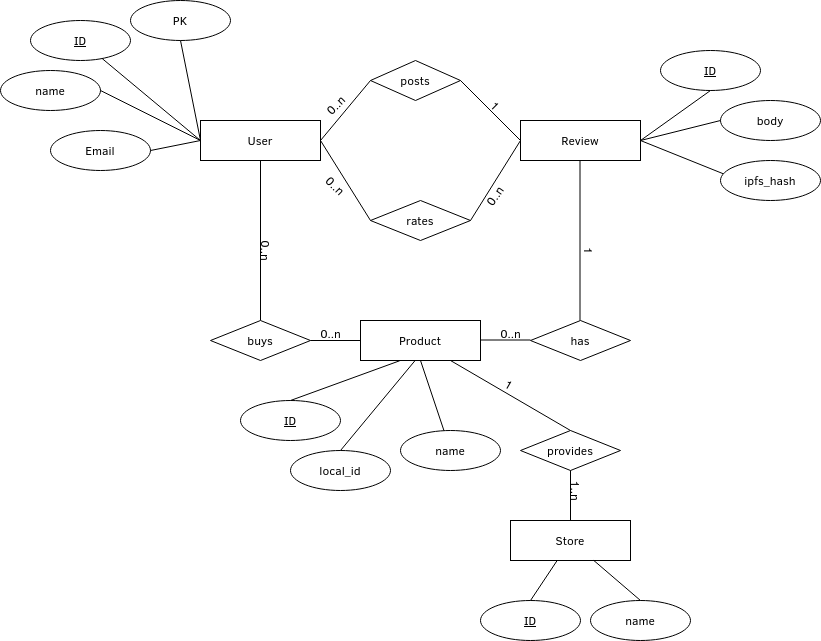
\includegraphics[width=0.6\linewidth]{figures/derp_er.drawio.png}
	\caption{Entity-Relationship diagram for the backend}
	\label{fig:er-diagram}
\end{figure}

To keep things organized, we created 4 Elixir contexts:
\begin{itemize}
	\item \textbf{Accounts}: procedures related to user authentication.
	\item \textbf{Catalogue}: procedures related to stores/products.
	\item \textbf{Reviews}: procedures related to reviews.
	\item \textbf{Oracle}: procedures related to the oracle.
\end{itemize}

The contexts for Accounts, Catalogue and Reviews handle the usual CRUD operations (which weren't really needed as we fetch data from chain).
The context for the Oracle is the most complex, as it has to spawn 2 subprocesses that listen for events from the contract and it allows us to grant review tokens to the users that request them after buying a product from the shop. The 2 subprocesses are handled by elixir and will restart on their own if they crash.

Here we include the (significant parts of the) oracle code.

\begin{figure}[H]
	\begin{minted}
defmodule Derp.Oracle.EventHandler do
  use Supervisor

  # Start process supervisor tree to check if we get new requests
  def start_link(_args) do
    Supervisor.start_link(__MODULE__, [], name: __MODULE__)
  end

  def init(_init_arg) do
    # Load contract and initialize it

    contract_abi = ExW3.Abi.load_abi("assets/js/Derp-abi.json")
    ExW3.Contract.start_link()
    ExW3.Contract.register(:Derp, abi: contract_abi)
    ExW3.Contract.at(:Derp, Application.fetch_env!(:derp, :contract_address))

    children = [
      __MODULE__.ReviewTokenRequest,
      __MODULE__.AllReviewTokenRequest
    ]

    Supervisor.init(children, strategy: :one_for_one)
  end

  # ...
    \end{minted}
	\label{code:oracle-init}
	\caption{Initialization code for the supervisor tree of the oracle. It starts two processes (``tasks'') that asynchronously check for incoming review request events emitted from a reviewer.}
\end{figure}

\begin{figure}[H]
	\begin{minted}{elixir}
defmodule Derp.Oracle.EventHandler do
  # ...

  defmodule AllReviewTokenRequest do
    use Task, restart: :permanent

    def start_link(_arg) do
      {:ok, filter_id} = ExW3.Contract.filter(:Derp, "AllReviewTokensRequested")

      state = [
        filter_id: filter_id
      ]

      Task.start_link(__MODULE__, :run, [state])
    end

    def run(state) do
      filter_id = state[:filter_id]
      {:ok, changes} = ExW3.Contract.get_filter_changes(filter_id)
      handle_changes(changes)
      :timer.sleep(1000)
      run(state)
    end

    # ...

    def handle_changes(changes) do
      Enum.each(changes, fn c ->
        address =
          ExW3.Address.from_bytes(c["data"]["account"])
          |> ExW3.Address.to_hex()

        Derp.Oracle.refresh_reviews_for_user(address, [])
      end)
    end
  end
    \end{minted}
	\label{code:all-review-token-request}
	\caption{Task that checks for review token requests for products which are not known. In this case the backend asks the external shops for the transaction history of the user and compares it to the state on-chain, to know if there are new products and accordingly reward the user the review tokens.}
\end{figure}

\begin{figure}[h]
	\begin{minted}{elixir}
defmodule Derp.Oracle do
  # ...

  def create_review_request(attrs \\ %{}) do
    changeset =
      %ReviewRequest{}
      |> ReviewRequest.create_changeset(attrs)

    address = changeset.changes.address
    products = changeset.changes.products || []

    if should_user_pay_request?(ReviewRequest, address) do
      {:error, :review_token_already_requested}
    else
      case refresh_reviews_for_user(address, products) do
        {:ok, true} ->
          Repo.insert_or_update(changeset)
          {:ok, true}

        error ->
          error
      end
    end
  end
  
  # ...
    \end{minted}
	\label{code:create-review-request}
	\caption{Code that checks for new products, reward the user their review tokens and register it on the database if they didn't do a daily review request beforehand.}
\end{figure}

\begin{figure}[H]
	\begin{minted}{elixir}
  def should_user_pay_request?(table, address) do
    now = DateTime.utc_now()
    day_start = %DateTime{now | hour: 0, minute: 0, second: 0}
    day_end = %DateTime{now | hour: 23, minute: 59, second: 59}

    query =
      from r in table,
        select: r.address,
        where:
          r.address == ^address and
            r.updated_at >= ^day_start and
            r.updated_at <= ^day_end

    Repo.exists?(query)
  end
    \end{minted}
	\label{code:request-check}
	\caption{Code that checks if the user did a review token request.}
\end{figure}


\begin{figure}[H]
	\begin{minted}{elixir}
  defp get_bought_products_from_store(address, 0) do
    Logger.info("Trying to check if #{address} bought new products...")

    store_url = "localhost:8080/check"
    headers = [{"Content-Type", "application/json"}]

    with {:ok, json} <- Jason.encode(%{address: address})
         {:ok, response} <- HTTPoison.post(store_url, json, headers),
         {:ok, %{"data" => result}} <- Jason.decode(response.body) do
      result
    else
      error -> error
    end 
  end

  def check_new_bought_products(address) do
    products =
      get_bought_products_from_store(address, 0)
      |> Enum.map(fn p -> 
        (0 <<< 32) ||| p
      end)

    {:ok, int_address} = ExW3.Utils.hex_to_integer(address)

    {:ok, claimedProducts} = ExW3.Contract.call(:Derp, :getClaimedProductsFromAccount, [int_address])

    products -- claimedProducts
  end

  # Request all tokens for all products
  def refresh_reviews_for_user(address, []) do
    Logger.info("Refreshing tokens for #{address}...")
    case check_new_bought_products(address) do
      [] -> {:error, :no_new_products}
      products when is_list(products) ->
        Derp.Oracle.reward_review_tokens(address, products)
      _error -> {:error, :no_new_products}
    end
  end
    \end{minted}
	\label{code:new-products-check}
	\caption{Functions that check if the user bought new products that we don't know about. By default we check just our store (ID 0). If there are new products, we grant review tokens to the user.}
\end{figure}

\begin{figure}[H]
	\begin{minted}{elixir}

  def decode_product_id(product) do
    store_id = (product &&& 0xFFFFFFFF <<< 32) >>> 32
    product_id = product &&& 0xFFFFFFFF

    {store_id, product_id}
  end

  def reward_review_tokens(address, product) do
    options = %{
      from: Enum.at(ExW3.accounts(), 0),
      gas: 1_000_000
    }

    {:ok, int_address} = ExW3.Utils.hex_to_integer(address)

    {store_id, local_product_id} = Derp.Oracle.decode_product_id(product)

    case ExW3.Contract.send(:Derp, :rewardReviewToken, [int_address, product], options) do
      {:ok, result} ->
        Logger.info(
          "Rewarded user #{address} for product #{product} (#{store_id}, #{local_product_id})"
        )

        {:ok, result}
    end
  end
    \end{minted}
	\label{code:review-token-reward}
	\caption{Code that actually rewards the user with review tokens for purchasing one or more products. The server pays for this transaction.}
\end{figure}

\paragraph{Why use a backend at all?} A case could be made that the backend is not really needed, as we could just use the smart contract to store all the data. However we do not need to verify the authenticity of all of the information used in the website (we mentioned user settings or preferences), and storing it on the chain would increase the price of the contract without any real benefit.
The backend also serves as a way to absorb part of the cost for the users that want to use the platform; for example it pays the transaction for registering the products and rewarding review tokens so that the user just pays for making reviews, upvoting other reviews, buying profile NFTs and requesting review tokens.
Additionally, having a solid (pun intended) backend is a good choice for future development, as it gives the possibility to easily expand the website in the future.

\subsection{Frontend}

The frontend for D.E.R.P. uses the Phoenix framework to render each webpage. To provide a better interaction, we also used Alpine.js  to handle events or refreshes and to fill data that was fetched from the contract or IPFS. We interacted with the smart contract through web3.js whenever a user had to make a transaction. For what regards the UI, we created a really basic design using Bootstrap 5.

\begin{figure}[H]
	\begin{minted}{javascript}
document.addEventListener('alpine:init', () => {
    Alpine.data('reviewData', () => ({
        reviews: [ ],

        // ...

        async refresh() {
          const reviewHashes = await contract.methods.getReviews().call();

          this.reviews.length = 0;
          for (i = 0; i < reviewHashes.length; i++) {

            const asciiAddress = web3.utils.hexToAscii(reviewHashes[i])
            const stream = await ipfs.cat(asciiAddress);

            const decoder = new TextDecoder()
            let data = ''

            for await (const chunk of stream) {
              // chunks of data are returned as a Uint8Array, convert it back to a string
              data += decoder.decode(chunk, { stream: true })
            }

            const json_data = JSON.parse(data);

            this.reviews.push({
              product_id: json_data.productNumber,
              title: json_data.reviewTitle,
              body: json_data.reviewBody,
              upvotes: 1,
            });
          }
        },
    \end{minted}
	\label{code:js-alpine}
	\caption{Example of using Alpine with Web3.js and IPFS. This automatically updates the DOM when the \texttt{reviews} variable is modified.}
\end{figure}

\subsection{Smart contract}

The smart contract for D.E.R.P. is written in Solidity and it is deployed on Truffle Suite. The main responsibilities of the contract are meant to fullfil most of the functional and non-functional requirements, namely:
\begin{itemize}
	\item store the reviews on-chain, grant authenticity \nreqref{nreq:security};
	\item store the products and some information about them \reqref{req:browse-products};
	\item store information about profile items and their prices \reqref{req:buy-items};
	\item handle users' interaction with products (e.g. verify that a user has bought a product or claimed their review tokens) \reqref{req:interact};
	\item handle the interactions regarding review tokens and profile tokens \reqref{req:interact}.
\end{itemize}

To complete the interaction with the smart contract we also used IPFS. In fact, storing the reviews on-chain would be too expensive, so we decided to store them on IPFS and just store the hash. This way, we can verify the authenticity of the review and we can also retrieve the review text easily. We did a similar thing for the profile items too, in order to store less information on chain. \\

Here we listed the most important parts of the smart contract:

\begin{figure}[H]
    \begin{minted}{solidity}
contract Derp {
    // "Unclaimed" is the default state for a product. When an user buys it and
    // they request its review tokens then the product becomes Claimed.
    // After making a review the product becomes Reviewed.
    enum ProductState {
        UNCLAIMED,
        CLAIMED,
        REVIEWED
    }

    // The product for which an user wants to make a review.
    // This is indexed as a combination of the store ID and the product ID
    // local to that store.
    // "_initialized" is used for checking if a product exists.
    //
    // Example:
    //    store ID = 1,
    //    local product ID = 1,
    //    product ID = 0x100000001
    struct Product {
        bytes[] reviewHashes;
        bool _initialized;
    }

    function getClaimedProductsFromAccount(address account)
        public
        view
        returns (uint64[] memory)
    {
        uint256 maxProducts = 0;
        for (uint256 i = 0; i < registeredProducts.length; ++i) {
            uint64 pId = registeredProducts[i];
            if (productsClaimed[account][pId] == ProductState.CLAIMED) {
                ++maxProducts;
            }
        }

        uint64[] memory ret = new uint64[](maxProducts);
        uint256 retIdx = 0;
        for (uint256 i = 0; i < registeredProducts.length; ++i) {
            uint64 pId = registeredProducts[i];
            if (productsClaimed[account][pId] == ProductState.CLAIMED) {
                ret[retIdx] = pId;
                ++retIdx;
            }
        }

        return ret;
    }
    \end{minted}
    \label{code:sc-structs}
    % \caption{The structs and enums used in the code for storing products and
    % reviews. We use \texttt{\_initialized} for checking if something exists
    % beforehand inside the various functions.
    % The way the product ID is compressed is a way to reduce gas costs for
    % searches.}
\end{figure}

% \begin{figure}[H]
%     \begin{minted}{solidity}
%     // The deployer of the contract.
%     // Used to check the authenticity of the reviews.
%     address private owner;
%
%     // Mapping from the uint64 product ID to the stored products.
%     mapping(uint64 => Product) private products;
%
%     // Array used to retrieve all the products stored on-chain.
%     uint64[] private registeredProducts;
%
%     // Mapping of the products actually claimed by an user.
%     // Used to store on-chain the validity of the reviews.
%     mapping(address => mapping(uint64 => ProductState)) private productsClaimed;
%
%     // The NFTs that allow the user to make reviews on the site and upvote other
%     // reviews.
%     mapping(address => int64) private reviewTokens;
%
%     // Mapping from the IPFS' Content Identifier of the review to the actual
%     // review.
%     mapping(bytes => Review) private reviews;
%
%     // Mapping used for retrieving the IPFS' CIDs of the reviews made by an
%     // address.
%     mapping(address => bytes[]) private reviewsFromAddress;
%
%     \end{minted}
%     \label{code:sc-products-reviews-vars}
%     \caption{Variables used for keeping track of the products, their state and
%     the reviews made by the various users. The various mappings allow for
%     faster searches inside the contract, reducing gas cost for function calls
%     but trading it off with the initial deployment cost.}
% \end{figure}

% \begin{figure}[H]
%     \begin{minted}{solidity}
%     // Mapping for the profile NFTs used on the website.
%     mapping(address => int64) private profileTokens;
%
%     // Array used to retrieve all the profile items stored on-chain
%     // that can be bought with user tokens
%     // This could be expanded in the future with a struct
%     bytes[] private profileItems;
%
%     // Mapping with the price of profile items
%     mapping(bytes => int64) private profileItemPrices;
%
%     // Mapping with a list of item profile purchased by a user
%     mapping(address => bytes[]) private userProfileItems;
%
%     // Events emitted when an user wants to know if some review tokens can be
%     // obtained because they bought a product.
%     //
%     // ReviewTokensGranted is emitted when the response is affirmative.
%     event AllReviewTokensRequested(address account);
%     event ReviewTokenRequested(address account, uint64 product);
%     event ReviewTokensGranted(address account);
%
%     // Constants used by the contract
%
%     int8 public constant REVIEW_COST = 2;
%     int8 public constant REVIEW_REWARD = 1;
%     int8 public constant UPVOTE_COST = 2;
%     int8 public constant UPVOTE_REWARD = 1;
%     int8 public constant PER_PURCHASE_TOKENS = 10;
%     \end{minted}
%     \label{code:sc-profile-vars}
%     \caption{Variables for the profile.}
% \end{figure}


\begin{figure}[H]
    \begin{minted}{solidity}
    function requestAllReviewTokens() external {
        emit AllReviewTokensRequested(msg.sender);
    }

    function rewardReviewTokens(address account, uint64[] calldata productIds)
        external
        onlyOwner
    {
        for (uint256 i = 0; i < productIds.length; ++i) {
            uint64 pId = productIds[i];
            if (!products[pId]._initialized) {
                Product memory p = Product({
                    _initialized: true,
                    reviewHashes: new bytes[](0)
                });

                registeredProducts.push(pId);
                products[pId] = p;
            }

            if (productsClaimed[account][pId] == ProductState.UNCLAIMED) {
                productsClaimed[account][pId] = ProductState.CLAIMED;
                reviewTokens[account] += PER_PURCHASE_TOKENS;

                emit ReviewTokensGranted(account);
            }
        }
    }

    function upvoteReview(bytes calldata reviewHash) external {
        Review storage review = reviews[reviewHash];
        require(review._initialized, "Review doesn't exist");
        require(
            reviewTokens[msg.sender] >= UPVOTE_COST,
            "Not enough review tokens"
        );
        require(review.reviewer != msg.sender, "Can't upvote it's own review");

        reviewTokens[msg.sender] -= UPVOTE_COST;

        review.upvotes += 1;

        profileTokens[review.reviewer] += UPVOTE_REWARD;
    }
    \end{minted}
    \label{code:}
    \caption{}
\end{figure}


\begin{figure}[H]
    \begin{minted}{solidity}
    // Reviewer is msg.sender
    function makeReview(uint64 productId, bytes calldata reviewHash)
        external
        returns (bool)
    {
        require(reviewTokens[msg.sender] >= REVIEW_COST, "Not enough tokens");
        require(!reviews[reviewHash]._initialized, "Review already exists");

        // Stops the user from making reviews of products they have not claimed.
        require(
            productsClaimed[msg.sender][productId] == ProductState.CLAIMED,
            "Product not claimed or already reviewed"
        );

        // Avoids creating a review for a product that doesn't exist.
        require(products[productId]._initialized, "Product doesn't exist");

        Review memory r = Review({
            reviewer: msg.sender,
            upvotes: 1,
            _initialized: true
        });

        reviewsFromAddress[msg.sender].push(reviewHash);

        reviews[reviewHash] = r;
        products[productId].reviewHashes.push(reviewHash);

        reviewTokens[msg.sender] -= REVIEW_COST;
        profileTokens[msg.sender] += REVIEW_REWARD;

        productsClaimed[msg.sender][productId] = ProductState.REVIEWED;

        return true;
    }
    \end{minted}
    \label{code:}
    \caption{}
\end{figure}



% \inputminted{Solidity}{Derp.sol}


\subsection{Sequence diagrams}

Here it follows the sequence diagram for the most complex interaction in D.E.R.P.: the diagram shows the code execution when an user requests review tokens from the Web UI and they haven't spent their free daily refresh.

In case the user has spent their daily refresh, an identical interaction takes place except that the user now pays for by calling the \texttt{requestAllReviewTokens} function in the smart contract. At that point the Oracle (\texttt{AllReviewTokenRequest} task in \texttt{EventHandler}) intercepts the event, calls \texttt{refresh\_review\_for\_user} and such sub-call is the same.

\begin{figure}[H]
	\centering
	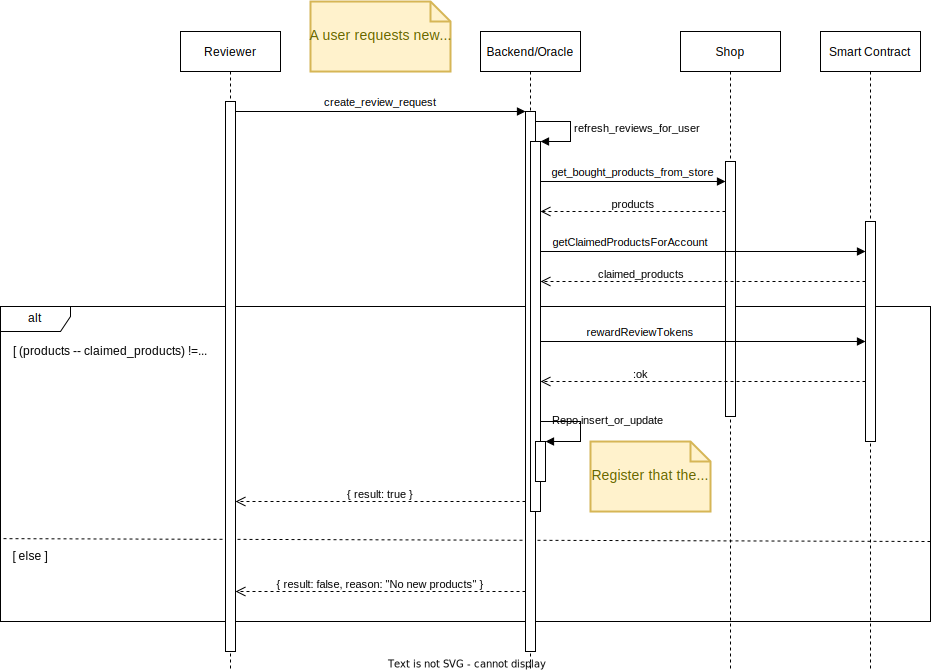
\includegraphics[width=0.9\linewidth]{figures/sd_review_token_request.pdf}
	\label{fig:sd-review-token-request}
	\caption{Sequence Diagram for the review token request.}
\end{figure}

\newpage

\subsection{Tokens lifecycle}

These are the lifecycle (activity) diagrams for the review and profile tokens.
It's possible to see that a user can actually choose how to spend their review tokens:
they can either make a review and/or upvote existing reviews from other users.
We don't stop the user from spending all their review tokens without making a review, however doing so will penalize them as this will decrease their possibility of receiving upvotes, thus profile tokens.

\begin{figure}[H]
	\centering
	\begin{minipage}{0.49\linewidth}
		\centering
		\includegraphics[width=0.75\linewidth]{figures/act-review-token-lc.pdf}
		\label{fig:act-review-token-lifecycle}
	\end{minipage}%
	\begin{minipage}{0.49\linewidth}
		\centering
		\includegraphics[width=0.75\linewidth]{figures/act-profile-token-lc.pdf}
		\label{fig:act-review-token-lifecycle}
	\end{minipage}
	\caption{The activity diagrams for the lifecycle of the review tokens (left) and the profile tokens (right).}
\end{figure}

To make the platform more engaging for the users, we decided to reward users 1 profile token for each upvote they receive on a review, while making upvotes cost 2 review tokens. Upon purchasing a product a user will receive 10 review tokens that equate to the ability to make a review for that product (using 2 review tokens) and upvoting 4 existing ones (using 2 review tokens for each).

\section{Images} %TO MOVE

\section{Known issues}

Our application has a number of known issues that stem from the very nature of the project. We will list them and try to provide a possible solution for each one:

\begin{itemize}
  \item {\bf{Oracle}}: the oracle is a single point of failure. If the oracle goes down, the application will not be able to function properly. We could solve this issue by using a distributed oracle, such as Chainlink. This would allow us to have multiple oracles that would be able to provide the same service, thus making the application more resilient to failures. 
  \item {\bf{OTC scams}}: the nature of the app makes it really expensive to make OTC scams, e.g. vendors making deals with customers outside the platform, but doesn't stop them completely. One way to fix this would be to rely on an e-commerce platform that implements a mechanism in which the customer cannot know the identity of the seller (while still being able to buy the product). This would make it impossible for the vendor to make deals with the customer outside the platform.
  \item {\bf{Review Bombing}}: the nature of the app makes it really hard to make review bombing attacks, e.g. a vendor making a lot of accounts and upvoting their own reviews. However, it doesn't stop them completely. 
  \item {\bf{API}}: e-commerces that want to use the platform are forced to implement an API which is compatible with our oracle. Furthermore, the API exposes some of the customers data to the public. This could be solved by using an e-commerce that implements similar protocols to our application - i.e. relies on the blockchain. Note that the current implementation would already work with blockchain based e-commerce.
\end{itemize}

\section{Conclusion}

\newpage
%\printbibliography


\end{document}

